\documentclass[t,11pt]{article}
% A modifier selon la personne...
\NeedsTeXFormat{LaTeX2e}




\RequirePackage{geometry}
\usepackage{beamerarticle}
%\usepackage{boxedminipage,multicol,pifont}
\renewcommand{\d}{\textrm{d}}
\renewcommand{\baselinestretch}{1.3}
\newcommand{\longueur}{6cm}
\RequirePackage{amsmath,amssymb}
\RequirePackage{amsfonts}
\RequirePackage{graphicx}
%\RequirePackage{mesmacros}
\usepackage[T1]{fontenc} 
\usepackage[utf8]{inputenc}
\usepackage[frenchb]{babel}
\usepackage{pifont}
\usepackage{lmodern}

\RequirePackage{comment}
\RequirePackage{multicol}

\RequirePackage{colortbl}
\RequirePackage{fancybox}
\usepackage{colortbl}


\RequirePackage{tikz,tkz-tab,tkz-fct,tkz-base,tkz-euclide}
%\RequirePackage{tikz,tkz-base,tkz-euclide}

%\RequirePackage{graphe}
\RequirePackage{framed}

\usepackage{ulem}
\normalem


%%%ENTETES%%%
%%%%%%%%%%%
\newcommand{\entetedebut}{
{\noindent \textbf{PTSI2 -- 2019/2020 -- Maths} \hfill Lycée La Martinière-Monplaisir -- Lyon \vspace{2mm}}
\hrule
\begin{center} 
}
\newcommand{\entetedebutinfo}{
{\noindent \textbf{PTSI -- 2023/2024 -- Info} \hfill Lycée La Martinière-Monplaisir -- Lyon \vspace{2mm} }
\hrule
\begin{center} 
}

\newcommand{\entetefin}{
\end{center}
\hrule
\vspace*{0.5cm}
}

\newcommand{\entetedebutsnow}{
\begin{tikzpicture}[decoration=Koch snowflake]
\draw (0,0)--(12,0)node[midway,above]
}

\newcommand{\entetefinsnow}{
\draw decorate{ decorate{ decorate{ decorate{ (12,0)--(17,0) }}}};
\end{tikzpicture}
\vspace*{1cm}
}
%%% Lorqu'on utilise les entetes koch snowflake, il faut juste mettre tout le titre entre { } et un point-virgule à la fin, car on est dans un tikzpicture.
\newcommand{\entetecours}{
\entetedebut
\textbf{\textsf{\Large Ch \numero. \titre.}}
\entetefin
}
\newcommand{\entetecoursinfo}{
\entetedebutinfo
\textbf{\textsf{\Large Ch \numero. \titre.}}
\entetefin
}


\newcommand{\entete}{
\entetedebut
\textbf{\textsf{\Large \titre.}}
\entetefin
}
\newcommand{\enteteinfo}{
\entetedebutinfo
\textbf{\textsf{\Large \titre.}}
\entetefin
}


\newcommand{\entetetd}{
\entetedebut
\textbf{\textsf{\Large TD \numero. \titre.}}
\entetefin
}

\newcommand{\entetetp}{
\entetedebut
\textbf{\textsf{\Large TP \numero. \titre.}}
\entetefin
}

\newcommand{\entetetpinfo}{
\entetedebutinfo
\textbf{\textsf{\Large TP \numero. \titre.}}
\entetefin
}



\newcommand{\enteteindic}{
\entetedebut
\textbf{\textsf{\Large Indications et solutions pour le TD \numero.}}
\entetefin
}


\newcommand{\entetecor}{
\entetedebut
\textbf{\textsf{\Large Corrigés pour le TD \numero.}}
\entetefin
}


%%%%%%%%%%%%%%%%%%%%%%%%%%%%%%%%%%%%%%%
\parindent=0pt

\newlength{\myline}


\newcommand{\graphetext}[3]{
\setlength{\myline}{\linewidth}
\addtolength{\myline}{-1cm}
\addtolength{\myline}{-#1}
\begin{tabular}{ll}
\parbox[c]{#1}{\includegraphics[width=#1]{#2}}&
\parbox[c]{\myline}{#3}
\end{tabular}}
\newcommand{\tikztexte}[3]{
\setlength{\myline}{\linewidth}
\addtolength{\myline}{-1cm}
\addtolength{\myline}{-#1}
\begin{tabular}{ll}
\parbox[c]{#1}{#2}&
\parbox[c]{\myline}{#3}
\end{tabular}}
\newcommand{\textgraphe}[3]{
\setlength{\myline}{\linewidth}
\addtolength{\myline}{-.5cm}
\addtolength{\myline}{-#1}
\begin{tabular}{ll}
\parbox[c]{\myline}{#2}&
\parbox[c]{#1}{\includegraphics[width=#1]{#3}}
\end{tabular}}
\newcommand{\textetikz}[3]{
\setlength{\myline}{\linewidth}
\addtolength{\myline}{-.5cm}
\addtolength{\myline}{-#1}
\begin{tabular}{ll}
\parbox[c]{\myline}{#2}&
\parbox[c]{#1}{#3}
\end{tabular}}
\newcommand{\p}{\pause}


%%%NUMEROTATION DES PARTIES%%%
\renewcommand{\thesection}{\hspace{-0.6cm}\arabic{section}}
\renewcommand{\thesubsection}{\hspace{-0.4cm}\arabic{section}.\alph{subsection}}
\renewcommand{\thesubsubsection}{\hspace{0cm}\arabic{section}.\alph{subsection}.\roman{subsubsection}}

%% Pour l'entete prof

\usepackage{fancyhdr}
\pagestyle{fancy}
\renewcommand{\headrulewidth}{0pt}
\fancyhead[L]{}
\fancyhead[R]{}
\fancyhead[C]{\blanc{\texttt{\tiny{\phantom{version prof - }version prof -  version prof - version prof - version prof - version prof - version prof - version prof - version prof}}}}


\definecolor{shadecolor}{gray}{0.9}

\newcommand{\espace}[1]{\vspace*{#1cm}}
\newcommand{\commentaire}[1]{}
\newcommand{\pourmoi}[1]{}
\newcommand{\bonly}[1]{}
\newcommand{\bexcept}[1]{#1}

\newcommand{\eleveonly}[1]{#1}

\newcommand{\gris}[1]{\textcolor{white}{#1}}




%%%%%%%%%%%%%%%%%%Numerotation%%%%%%%%%%%%%%%%%%

\renewcommand{\labelenumi}{\textbf{\arabic{enumi}${}^\circ$)}}
\renewcommand{\labelenumii}{\textbf{\alph{enumii})}}
%\renewcommand{\thesection}{\Roman{section}}
%\renewcommand{\thesubsection}{\Alph{subsection})}
%\renewcommand{\thesubsubsection}{\arabic{subsubsection})}

%\renewenvironment{itemiz}%
%{\begin{itemize}\renewcommand{\labelitemi}{\ding{51}}}
%{\end{itemize}}


%\newenvironment{itemiz}[1][84]% 117 81 71
%{\begin{dinglist}{#1}}
%{\end{dinglist}}

%\newenvironment{itemiz}[1][]
%{\begin{itemize} \itemsep5pt 
 %\renewcommand{\labelitemi}{\bubul}}
%{\end{itemize}}

\newenvironment{itemiz}[1][]%
{ \begin{list}%
	{\bubul}%
	{%\setlength{\labelwidth}{30pt}%
	 \setlength{\leftmargin}{20pt}%
	 \setlength{\itemsep}{4pt}}}%
{ \end{list} }


%%%%%%%%%%%%%%%%%%%%%%%Les encadrés%%%%%%%%%%%%%%%%
\newenvironment{python}
{\vspace{-0.2cm}\begin{shaded}\ttfamily}
{\normalfont\end{shaded}\vspace{0.2cm}}

\newenvironment{pythonshell}
{\begin{shaded}
\textit{Python shell}\\
\ttfamily}
{\normalfont\end{shaded}\vspace{0.2cm}}




%\newenvironment{defn}[1][]{\vspace{.2cm}
%\begin{minipage}{\linewidth}
%{\bf Définition\vphantom{p} : #1}
%\newline
%\noindent
%\begin{boxedminipage}{\linewidth}}{
%\end{boxedminipage}\vspace{.5cm}\end{minipage}}

%\newenvironment{defn}[1][]{\vspace{.2cm}
%\begin{minipage}{\linewidth}
%{\bf Définition\vphantom{p} : #1}
%\newline
%\noindent
%\begin{boxedminipage}{\linewidth}}{
%\vspace{.05cm}\end{boxedminipage}\vspace{0.2cm}\end{minipage}}

\newcommand{\debutprop}{\newline
\hspace*{5mm}
\begin{tikzpicture}
  \node[rectangle,inner sep=0pt,outer sep=10pt]%
  (A)  \bgroup
    \begin{minipage}{0.9\linewidth}
    }
    
\newcommand{\finprop}{
    \end{minipage}
    \egroup;
\draw (A.north west) -- (A.south west) ;
\draw (A.south west) -- (A.south east) ;
%\draw (A.north west) -- (A.north east) ;
%\draw (A.north east) -- (A.south east) ;
\end{tikzpicture}\\
}

\newenvironment{defn}[1][]
{\textbf{Définition\vphantom{p} : #1}\debutprop
      }
     {\finprop
}


%\newenvironment{cor}[1][]{\vspace{.2cm}
%\begin{minipage}{\linewidth}
%{\bf Corollaire\vphantom{p} : #1}
%\newline
%\noindent
%\begin{boxedminipage}{\linewidth}}{
%\vspace{.05cm}\end{boxedminipage}\vspace{0.2cm}\end{minipage}}

\newenvironment{cor}[1][]
{\textbf{Corollaire\vphantom{p} : #1}\debutprop}
     {\finprop}

%\newenvironment{lemme}[1][]{\vspace{.2cm}
%\begin{minipage}{\linewidth}
%{\bf Lemme\vphantom{p} : #1}
%\newline
%\noindent
%\begin{boxedminipage}{\linewidth}}{
%\vspace{.05cm}\end{boxedminipage}\vspace{0.2cm}\end{minipage}}

\newenvironment{lemme}[1][]
{\textbf{Lemme\vphantom{p} : #1}\debutprop}
     {\finprop}


%\newenvironment{theo}[1][]{\vspace{.2cm}
%\begin{minipage}{\linewidth}
%{\bf ThéorÚme \vphantom{p}: #1}
%\newline
%\noindent
%\begin{boxedminipage}{\linewidth}}{
%\vspace{.05cm}\end{boxedminipage}\vspace{0.2cm}\end{minipage}}

\newenvironment{theo}[1][]
{\textbf{Théorème\vphantom{p} : #1}\debutprop}
     {\finprop}
     
     \newenvironment{theodefn}[1][]
{\textbf{Théorème-définition\vphantom{p} : #1}\debutprop}
     {\finprop}


%\newenvironment{propdef}[1][]{\vspace{.2cm}
%\begin{minipage}{\linewidth}
%{\bf Proposition et définition : #1}
%\newline
%\noindent
%\begin{boxedminipage}{\linewidth}}{
%\vspace{.05cm}\end{boxedminipage}\vspace{0.2cm}\end{minipage}}

\newenvironment{propdef}[1][]
{\textbf{Proposition-définition\vphantom{p} : #1}\debutprop}
     {\finprop}

%\newenvironment{prop}[1][]{\vspace{.2cm}\noindent
%\begin{minipage}{\linewidth}{\bf Proposition : #1}
%\newline
%\noindent
%\begin{boxedminipage}{\linewidth}}{
%\vspace{.05cm}\end{boxedminipage}\vspace{0.2cm}\end{minipage}}

\newenvironment{prop}[1][]
{\textbf{Proposition\vphantom{p} : #1}\debutprop}
     {\finprop}

\newenvironment{rem}[1][]{\vspace{.2cm}\noindent\begin{minipage}{\linewidth}{\bf Remarque : #1}\newline\noindent}{\end{minipage}\vspace{.5cm}}
\newenvironment{meth}[1][]{\vspace{.2cm}\noindent\begin{minipage}{\linewidth}{\bf Méthode : #1}\newline\noindent}{\end{minipage}\vspace{.5cm}}
\newenvironment{rems}[1][]{\vspace{.2cm}\noindent\begin{minipage}{\linewidth}{\bf Remarques : #1}\noindent}{\end{minipage}\vspace{0.5cm}}
\newenvironment{remnum}[1]{\vspace{.2cm}\noindent\begin{minipage}{\linewidth}{\bf Remarque #1 : }\newline\noindent}{\end{minipage} \vspace{.5cm}}
\newenvironment{exe}[1][]{\vspace{0.2cm}\noindent\begin{minipage}{\linewidth}{\bf Exemple : #1}\newline\noindent}{\end{minipage}\vspace{.5cm}}
\newenvironment{exes}[1][]{\vspace{0.2cm}\noindent\begin{minipage}{\linewidth}{\bf Exemples : #1}\noindent}{\end{minipage}\vspace{0.5cm}}
\newenvironment{exenum}[1]{\vspace{.2cm}\noindent\begin{minipage}{\linewidth}{\bf Exemple #1 : }\newline\noindent}{\end{minipage}\vspace{.5cm}}
\newenvironment{nota}[1][]{\vspace{.2cm}\noindent\begin{minipage}{\linewidth}{\bf Notation : #1}\newline\noindent}{\end{minipage}\vspace{.5cm}}
\newcounter{ndem}
\setcounter{ndem}{0}
\newcommand{\dem}{\stepcounter{ndem}{\includegraphics{crayon5} \ \textbf{Démonstration} \thendem }\vspace{.5cm}}



%%% numerotation des questions exo
\newcounter{cexo}
\newenvironment{qexo}{
\refstepcounter{cexo}
\vspace{3 pt}
\noindent
\begin{minipage}[t]{0.15\textwidth}
\textbf{\noindent Question \arabic{cexo}. }
\end{minipage}\noindent
\begin{minipage}[t]{0.85\textwidth}}{\vspace{3 pt}
\end{minipage}}%\vspace{2 pt}


\usepackage{multicol}
\usepackage{ulem}
\normalem

\parindent=0pt

\RequirePackage{framed}

\graphicspath{{images_archi_materielle/}{images_archi_logicielle/}}
\newcommand{\FIG}[1]{\textsc{Figure} {\upshape\ref{#1}}}
\usepackage{numprint} %affichage de nombres correctement avec \numprint{}

%\usepackage{picins}    %permet d'insérer une image à coté d'un texte \parpic[r]{\includegraphics{}}texte...
\usepackage{tikz}
\usetikzlibrary{calc}
% Unités
\usepackage[locale = FR]{siunitx}
\sisetup{inter-unit-product = \ensuremath{{}\cdot{}}}
\usepackage{numprint} %affichage de nombres correctment avec \numprint{}
\usepackage{multirow}
\definecolor{gris_c}{gray}{0.9}
\definecolor{gris_f}{gray}{0.25}
\definecolor{gris_tc}{gray}{0.96}
\definecolor{gris_ttc}{gray}{0.98}

%%% activite
\newenvironment{activite}[1][\hsize]%
{%
    \def\FrameCommand%
    {%
\rotatebox{90}{\textit{\textsf{REMARQUE}}} 
        {\color{blue}\vrule width 3pt}%
        \hspace{0pt}%must no space.
        \fboxsep=\FrameSep\colorbox{gris_c}%
    }%
    \MakeFramed{\hsize#1\advance\hsize-\width\FrameRestore}%
}%
{\endMakeFramed}%


%%% objectif
\newenvironment{objectif}[1][\hsize]%
{%
    \def\FrameCommand%
    {%
\rotatebox{90}{\textit{\textsf{OBJECTIF}}} 
        {\color{blue}\vrule width 3pt}%
        \hspace{0pt}%must no space.
        \fboxsep=\FrameSep\colorbox{gris_c}%
    }%
    \MakeFramed{\hsize#1\advance\hsize-\width\FrameRestore}%
}%
{\endMakeFramed}%

%%%%exos TP Info



\newtheorem{Exc}{Exercice}
\def\exotp#1{\futurelet\testchar\MaybeOptArgmyexoo}
\def\MaybeOptArgmyexoo{\ifx[\testchar \let\next\OptArgmyexoo
                        \else \let\next\NoOptArgmyexoo \fi \next}
\def\OptArgmyexoo[#1]{\begin{Exc}[#1]\normalfont}
\def\NoOptArgmyexoo{\begin{Exc}\normalfont}
\newcommand{\finexotp}{\end{Exc}}

\theoremstyle{definition}
\newtheorem{exo}{Exercice}

\usetikzlibrary{decorations.fractals}
\usetikzlibrary{matrix}

\newcommand{\cache}[1]{\phantomchoix{#1}\hspace{1.5cm}}
\newcommand{\Cache}[1]{\vspace*{0.2cm}\phantomchoix{\begin{minipage}{\linewidth}{#1}\end{minipage}}\vspace*{0.5cm}}

\newcommand{\indente}{\hspace*{1cm}}
\newcommand{\invite}{{>}{>}{>} }


\renewcommand{\vec}[1]{\overrightarrow{#1}}
\newcommand{\B}{\mathcal{B}}
\renewcommand{\P}{\mathcal{P}}
\renewcommand{\epsilon}{\varepsilon}
\newcommand{\A}{\mathcal{A}}
\newcommand{\re}{\mathcal{R}}

\newcommand{\un}{{1\!\mbox{l}}}
\newcommand{\E}{\mathbb{E}}
\newcommand{\R}{\mathbb{R}}
\newcommand{\Z}{\mathbb{Z}}
\newcommand{\Q}{\mathbb{Q}}
\newcommand{\N}{\mathbb{N}}
\newcommand{\C}{\mathbb{C}}
\newcommand{\U}{\mathbb{U}}
\newcommand{\cc}{\small{\mathbb{c}}}
\newcommand{\F}{\mathcal{F}}
\newcommand{\K}{\mathbb{K}}
% Commande \tend :
% bla \tend{n}{l} bli :
%
%      bla   ->   bli
%          n -> l
%
%\newcommand{\tend}[2]{{\atop\stackrel{\displaystyle\longrightarrow}{\scriptstyle{{#1} \rightarrow {#2}}}}}
\newcommand{\tend}[2]{\underset{#1 \rightarrow #2}{\longrightarrow}}
\renewcommand{\o}[1]{\underset{#1}{o}}
%\renewcommand{\O}[1]{\underset{#1}{O}}
\DeclareMathOperator{\Det}{Det}

\newcommand{\Max}[1]{\underset{#1}{\max}\ }
\newcommand{\Min}[1]{\underset{#1}{\min}\ }
\newcommand{\Inf}[1]{\underset{#1}{\inf}\ }
\newcommand{\Sup}[1]{\underset{#1}{\sup}\ }
\newcommand{\Lim}[1]{\underset{#1}{\lim}\ }
\newcommand{\Sim}[1]{\underset{#1}{\sim}\ }
\def\det{\mathop{\operator@font det}\nolimits}
\def\Tr{\mathop{\operator@font Tr}\nolimits}
\def\Card{\mathop{\operator@font Card}\nolimits}
%\def\Ker{\mathop{\operator@font Ker}\nolimits}
\newcommand{\Ker}{\textrm{Ker}}
\newcommand{\Vect}{\textrm{Vect}}
\def\rg{\mathop{\operator@font rg}\nolimits}
\def\Im{\mathop{\operator@font Im}\nolimits}
\def\Re{\mathop{\operator@font Re}\nolimits}
%\def\Arg{\mathop{\operator@font Arg}\nolimits}
\def\Argsh{\mathop{\operator@font Argsh}\nolimits}
\def\Argch{\mathop{\operator@font Argch}\nolimits}
\def\Argth{\mathop{\operator@font Argth}\nolimits}
%\def\cotan{\mathop{\operator@font cotan}\nolimits}
\def\Arctan{\mathop{\operator@font Arctan}\nolimits}
\def\Arccos{\mathop{\operator@font Arccos}\nolimits}
\def\Arcsin{\mathop{\operator@font Arcsin}\nolimits}
\def\Argcoth{\mathop{\operator@font Argcoth}\nolimits}
%\def\sh{\mathop{\operator@font sh}\nolimits}
\def\coth{\mathop{\operator@font coth}\nolimits}
\def\tanh{\mathop{\operator@font th}\nolimits}
%\def\ch{\mathop{\operator@font ch}\nolimits}
\def\div{\mathop{\operator@font div}\nolimits}
\def\rot{\mathop{\overrightarrow{\operator@font rot}}\nolimits}
\def\grad{\mathop{\overrightarrow{\operator@font grad}}\nolimits}

\def\card{\mathop{\operator@font card}\nolimits}
\newcommand{\scal}[2]{\langle #1 | #2 \rangle}
\newcommand{\norme}[1]{\| #1 \|}
%\newcommand{\ang}[1]{\sphericalangle #1}

\newcommand{\fonc}[4]{\begin{array}[t]{rcl}
#1&\rightarrow&#2\\
#3&\mapsto&#4\end{array}}

%\newcommand{\soupoint}[1]{\d}
\renewcommand{\d}{\,\textrm{d}}
%\renewcommand{\d}{\operatorname{d}\!}
\newcommand{\der}[3][]{\dfrac{\textrm{d}^{#1} #2}{\textrm{d} #3^{#1}}}
\newcommand{\derpar}[3][]{\dfrac{\partial^{#1} #2}{\partial #3^{#1}}}
\newcommand{\dercroise}[3]{\dfrac{\partial^{2}#1}{\partial#2\partial#3}}
\newcommand{\doubleint}{\int\!\!\!\int}
\newcommand{\tripleint}{\int\!\!\!\int\!\!\!\int}

\newcommand{\D}[1]{\displaystyle{#1}}

\renewcommand{\bar}{\overline}




%%%Delphine%%%
%%%COMMANDES PRATIQUES%%%
%%%GENERAL%%%
\newcommand{\bubul}{$\bullet$ }
\newcommand{\qqsoit}{\forall \,}
\newcommand{\ilex}{\exists \,}
\newcommand{\di}{\displaystyle}
\newcommand{\ep}{\varepsilon}
\renewcommand{\l}{\lambda}
\newcommand{\ssi}{\Longleftrightarrow}
%\newcommand{\sensdirect}{\fbox{$\Rightarrow$} }
%\newcommand{\sensindirect}{\fbox{$\Leftarrow$} }
\newcommand{\li}{\begin{itemize}}
\newcommand{\finli}{\end{itemize}}
\newcommand{\syst}{\left\{\begin{array}{l}}
\newcommand{\finsyst}{\end{array} \right.}
\newcommand{\va}{|}
\newcommand{\plrs}{\begin{eqnarray*}}
\newcommand{\finplrs}{\end{eqnarray*}}
\newcommand{\Arg}{\text{Arg}}
\newcommand{\ent}[1]{\left\lfloor #1\right\rfloor}

%%%PROBAS%%%
%\DeclareMathOperator{\card}{Card}
%\newcommand{\E}{\mathbb{E}}    
%\renewcommand{\P}{\mathbb{P}}  
\newcommand{\cov}{\text{cov}}  

%%%ANALYSE%%%
\providecommand{\abs}[1]{\left\lvert#1\right\rvert} %valeur absolue
\providecommand{\fonction}[5]
    {\begin{array}[t]{cccl}#1  : & #2&\rightarrow&#3\\{} & #4&\mapsto&#5\end{array}}
\providecommand{\eq}[2]{\underset{#1 \rightarrow #2}{\sim}}
\providecommand{\tend}[2]{\underset{#1 \rightarrow #2}{\longrightarrow}}
\providecommand{\limite}[2]{\displaystyle \lim_{#1 \rightarrow #2}}
\providecommand{\dl}[2]{\underset{#1 \rightarrow #2}{=}}
%\renewcommand{\d}{\operatorname{d}}
\newcommand{\drond}{\partial}
\renewcommand{\i}{\operatorname{i}}
\newcommand{\ch}{\operatorname{ch}}
\newcommand{\sh}{\operatorname{sh}}
\renewcommand{\th}{\operatorname{th}}
\newcommand{\cotan}{\operatorname{cotan}}
\renewcommand{\arctan}{\operatorname{Arctan}}
\renewcommand{\arcsin}{\operatorname{Arcsin}}
\renewcommand{\arccos}{\operatorname{Arccos}}
\newcommand{\argth}{\operatorname{argth}}
\newcommand{\argsh}{\operatorname{argsh}}
\newcommand{\argch}{\operatorname{argch}}
\renewcommand{\Re}{\text{Re}}
\renewcommand{\Im}{\text{Im}}

%%%ALGEBRE%%%
\providecommand{\norm}[1]{\left\rVert#1\right\rVert} %norme
\providecommand{\sdo}[0]{\text{\odplus}} % somme directe orthogonale
\renewcommand{\ker}{\operatorname{Ker}}
%\newcommand{\Ker}{\operatorname{Ker}}
%\renewcommand{\o}{\operatorname{o}}
\renewcommand{\O}{\operatorname{O}}
\newcommand{\trans}{\,{}^{\text{t}}} % transposée
\DeclareMathOperator{\tr}{tr}  %trace
%\DeclareMathOperator{\im}{\text{Im}}
\newcommand{\im}{\operatorname{Im}}
\DeclareMathOperator{\id}{id}
\providecommand{\mat}[1]{\underset{#1}{\text{mat}}}
\DeclareMathOperator{\vect}{\text{Vect}}
%\DeclareMathOperator{\rg}{\text{rg}}


%%%MAPLE%%%
\newenvironment{prog}{ \color{red}\ttfamily}{\color{black}}
\newcommand{\maple}{\begin{prog}}
\newcommand{\finmaple}{\end{prog}}
\newenvironment{reponse}{ \begin{center}  \color{blue} \em}{\end{center}\color{black}}
\newcommand{\rep}{\begin{reponse}}
\newcommand{\finrep}{\end{reponse}}


%%%GEOMETRIE%%%
\providecommand{\vecteur}[1]{\overrightarrow{#1}}

%%DIVERS%%
%\newcommand{\s}{ $ }
%\newcommand{\ds}{ $$ }
\newcommand{\itbul}{\item[\bubul]}

%\usepackage{tikz,tkz-tab}
%\usepackage[babel=true,kerning=true]{microtype}

\tikzset{math3d/.style={x={(-0.353cm,-0.353cm)},z={(0cm,1cm)},y={(1cm,0cm)}}}

\tikzset{
xmin/.store in=\xmin, xmin/.default=-3, xmin=-3,
xmax/.store in=\xmax, xmax/.default=3, xmin=3,
ymin/.store in=\ymin, ymin/.default=-3, ymin=-3,
ymax/.store in=\ymax, ymax/.default=-3, ymax=-3,
}
\newcommand{\grille}{\draw[help lines] (\xmin,\ymin) grid (\xmax,\ymax);}

\newcommand{\axes}{%
\draw[->] (\xmin,0)--(\xmax,0);
\draw[->] (0,\ymin)--(0,\ymax);
\draw[->][very thick] (0,0)--(1,0);
%\draw (1 , 0) node[below] {$1$};
%\draw (0.5 , 0) node[below] {$\vec{i}$};
\draw (0.5 , 0) node[below] {$\vec{\imath}$};
\draw[->] [very thick](0,0)--(0,1);
%\draw (0,0.5) node[left] {$\vec{j}$};
\draw (0 , 0.5) node[left] {$\vec{\jmath}$};
%\draw (0,1) node[left] {$1$};
%\draw (0,0) node[below left]{$O$};
}

\newcommand{\axesbis}{%
\draw[->] (\xmin,0)--(\xmax,0)node[below]{$x$};
\draw[->] (0,\ymin)--(0,\ymax)node[left]{$y$};
}

\newcommand{\fenetre}
{\clip (\xmin,\ymin) rectangle (\xmax,\ymax);}

\newcommand{\repere}{%
\tikzset{xaxe style/.style={-}}
\tikzset{yaxe style/.style={-}}
\tkzInit[xmin=\xmin,xmax=\xmax,ymin=\ymin,ymax=\ymax]
\tkzDrawX[noticks]\tkzDrawY[noticks]
\tkzRep
}

\newcommand{\attention}{\raisebox{-2pt}{\includegraphics[width=5mm]{/Users/Delphine/1.BOULOT/2019_2020_PTSI_info/attention}}\ }

\usepackage{hyperref}
\hypersetup{
    colorlinks=true,
    linkcolor=blue,
    filecolor=magenta,      
    urlcolor=cyan,
    pdftitle={Overleaf Example},
    pdfpagemode=FullScreen,
    }

%%% Python
\usepackage{listingsutf8}
\lstset{language=Python,
  inputencoding=utf8/latin1,
  breaklines=true,
  basicstyle=\ttfamily\small,
  keywordstyle=\bfseries\color{green!40!black},
  commentstyle=\itshape\color{purple!40!black},
  identifierstyle=\color{blue},
  stringstyle=\color{orange},
  upquote = true,
  columns=fullflexible,
  backgroundcolor=\color{gray!10},frame=leftline,rulecolor=\color{gray}}  
  

\lstset{
     literate=%
         {é}{{\'e}}1    
         {è}{{\`e}}1    
         {ê}{{\^e}}1    
         {à}{{\`a}}1    
         {ô}{{\^o}}1    
         {ù}{{\`u}}1    
}

%%% Exemple
\newenvironment{exemple}[1][\hsize]%
{%
    \def\FrameCommand%
    {%
\rotatebox{90}{\textit{\textsf{Exemple}}} 
        {\color{blue}\vrule width 3pt}%
        \hspace{0pt}%must no space.
        \fboxsep=\FrameSep\colorbox{gris_c}%
    }%
    \MakeFramed{\hsize#1\advance\hsize-\width\FrameRestore}%
}%
{\endMakeFramed}%


\newenvironment{defi}[1][]
{\textbf{Définition\vphantom{p} : #1}\debutprop}
     {\finprop}
     
\newenvironment{theoreme}[1][]
{\textbf{Théorème\vphantom{p} : #1}\debutprop}
     {\finprop}
     
\newenvironment{propriete}[1][]
{\textbf{Propriété\vphantom{p} : #1}\debutprop}
     {\finprop}     

\newenvironment{comp}[1][]
{\textbf{Complexité\vphantom{p} : #1}\debutprop}
     {\finprop}

\newenvironment{obje}[1][]
{\textbf{Objectifs\vphantom{p} : #1}\debutprop}
     {\finprop}

\newenvironment{ordre}[1][]
{\textbf{Ordre de grandeurs\vphantom{p} : #1}\debutprop}
     {\finprop}

\newenvironment{methode}[1][]
{\textbf{Méthode\vphantom{p} : #1}\debutprop}
     {\finprop}

%% Questions et exercices
\newcounter{numques}%Création d'un compteur qui s'appelle numques
\setcounter{numques}{0}%initialisation du compteur
\newcommand{\question}[1]{%Création d'une macro ayant un paramètre
\addtocounter{numques}{1}%chaque fois que cette macro est appelée, elle ajoute 1 au compteur numexos
\textbf{Question\, \textcolor{black}{\thenumques}\,}\,\textit{#1}\\{\vspace{0cm}}}



\geometry{a4paper,top=2cm,bottom=2cm,left=2cm,right=2cm}

% A modifier pour chaque chapitre...
\newcommand{\titre}{Graphe - le plus court chemin - Algorithme A Star}
\newcommand{\numero}{21bis}

% Prof ou élève...
% prof : 
%\newcommand{\phantomchoix}[1]{\textcolor{red}{#1}}
%\newcommand{\blanc}[1]{\textcolor{red}{#1}}
% eleve : 
\newcommand{\phantomchoix}[1]{\phantom{#1}}
\newcommand{\blanc}[1]{\textcolor{white}{#1}}
\newcommand{\bl}[1]{\textcolor{black}{#1}}

\renewcommand{\cache}[1]{\phantomchoix{#1}\hspace*{0.1mm}}

%%% utilisation des algorithmes
\usepackage{algorithm}
\usepackage{algorithmic}
\renewcommand{\algorithmicrequire} {\textbf{\textsc{Entrées:}}}
\renewcommand{\algorithmicensure}  {\textbf{\textsc{Sorties:}}}
\renewcommand{\algorithmicwhile}   {\textbf{tantque}}
\renewcommand{\algorithmicdo}      {\textbf{faire}}
\renewcommand{\algorithmicendwhile}{\textbf{fin tantque}}
\renewcommand{\algorithmicend}     {\textbf{fin}}
\renewcommand{\algorithmicif}      {\textbf{si}}
\renewcommand{\algorithmicendif}   {\textbf{finsi}}
\renewcommand{\algorithmicelse}    {\textbf{sinon}}
\renewcommand{\algorithmicthen}    {\textbf{alors}}
\renewcommand{\algorithmicfor}     {\textbf{pour}}
\renewcommand{\algorithmicforall}  {\textbf{pour tout}}
\renewcommand{\algorithmicdo}      {\textbf{faire}}
\renewcommand{\algorithmicendfor}  {\textbf{fin pour}}
\renewcommand{\algorithmicloop}    {\textbf{boucler}}
\renewcommand{\algorithmicendloop} {\textbf{fin boucle}}
\renewcommand{\algorithmicrepeat}  {\textbf{répéter}}
\renewcommand{\algorithmicuntil}   {\textbf{jusqu'à}}

\floatname{algorithm}{Algorithme}

\let\mylistof\listof
\renewcommand\listof[2]{\mylistof{algorithm}{Liste des algorithmes}}

% pour palier au problème de niveau des algos
\makeatletter
\providecommand*{\toclevel@algorithm}{0}
\makeatother

\begin{document}
\entetecoursinfo







\section{Problématique}

Lorsque l'on cherche le plus court chemin entre deux sommets, départ et arrivée, le plus rapidement possible et en évitant les obstacles éventuels, l'algorithme A* (prononcer A star) est fait pour ça ! Cet algorithme est principalement utilisé dans les jeux vidéos :

%\begin{center}
%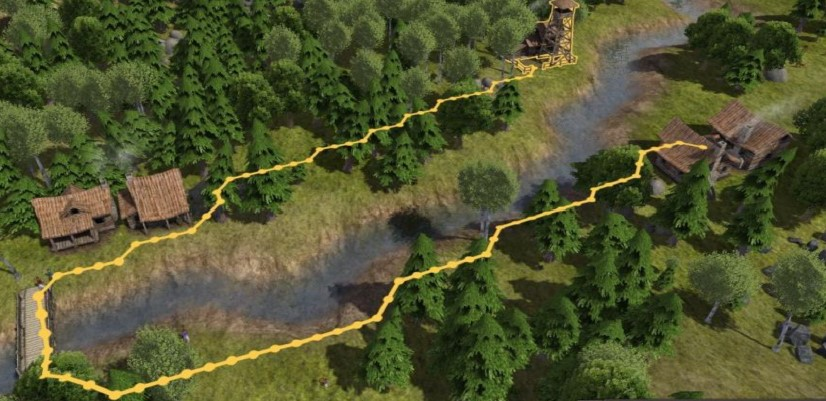
\includegraphics[scale=0.5]{images/jeuVideo.jpg}
%%\caption{Exemple de chemin}
%\end{center}

\begin{figure}[!h]
\centering
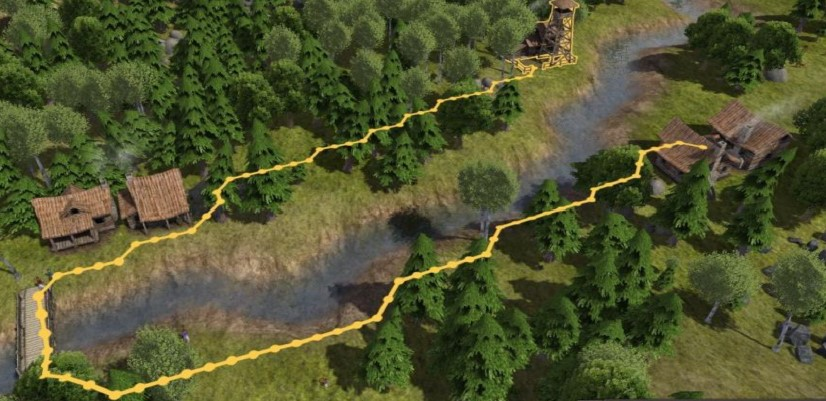
\includegraphics[scale=0.5]{images/jeuVideo.jpg}
\caption{Exemple de chemin}
\end{figure}

C'est un algorithme de recherche de chemin dans un graphe. C'est l'un des plus efficaces en la matière. Il ne donne pas toujours la solution optimale mais il donne très rapidement une bonne solution.\\
Au premier abord, on pourrait se dire que pour trouver un chemin d'un point à un autre il faut commencer par se diriger vers la destination. Et bien... c'est justement cette idée qu'utilise l'algorithme A* ! L'idée est très simple : à chaque itération, on va tenter de se rapprocher de la destination. Pour cela, on va donc privilégier les possibilités directement les plus proches de la destination, en mettant de côté toutes les autres. Toutes les possibilités ne permettant pas de se rapprocher de la destination sont mises de côté, mais pas supprimées. Elles
sont simplement mises dans une liste de possibilités à explorer si jamais la solution en cours s'avère mauvaise.
En effet, on ne peut pas savoir à l'avance si un chemin va aboutir ou s'il sera le plus court. Il suffit que ce chemin amène à une impasse pour que cette solution devienne inexploitable.\\
L'algorithme va donc d'abord se diriger vers les chemins les plus directs. Et si ces chemins n'aboutissent pas ou bien s'avèrent mauvais par la suite, il examinera les solutions mises de côté. C'est ce retour en arrière pour examiner les solutions mises de côté qui nous garantit que l'algorithme nous trouvera toujours une solution (si
tant est qu'elle existe, bien sûr).


\section{Comment fonctionne cet algorithme}

Il est basé sur l'algorithme de \texttt{Dijkstra} auquel est ajouté une \texttt{heuristique}.\\

En algorithmique, une heuristique est une méthode de calcul qui fournit rapidement une solution réalisable, pas nécessairement optimale ou exacte, pour un problème d'optimisation difficile (wikipédia).\\

Cette heuristique est définie dans la fonction :

$$f(s)=g(s)+h(s) $$

Avec :
\begin{itemize}
\item $g(s)$ est le coût du chemin optimal partant du sommet initial jusqu'au sommet $s$ ;
\item $h(s)$ le coût estimé du reste du chemin partant de $s$ jusqu'à un état satisfaisant de l'arrivée. $h(s)$ est une heuristique.
\end{itemize}

\subsection{Principe}

Dans des applications de recherche de chemin sur une image ou un quadrillage par exemple, il est possible de connaître pour chaque sommet la distance « à vol d'oiseau » ou « à taxi-distance » de chaque sommet à l'arrivée. On peut utiliser une de ces heuristiques et, au lieu de choisir le sommet ayant la plus petite distance depuis le départ parmi les sommets visités, on peut choisir la relation :
$$f(s)=d(depart,s)+d'(s,fin) $$

On choisit alors la valeur \texttt{min} des f(s) des sommets visités.

\textit{Remarque} : la valeur calculée peut être mémorisée sous forme d'entier (voir exemple).\\

Vous pouvez calculer ces distances de la manière que vous voulez, distance euclidienne, distance de \texttt{Manhattan} ou autre, elles peuvent convenir.\\
La distance de \texttt{Manhattan}, appelée aussi taxi-distance, est la distance entre deux points parcourue par un taxi lorsqu'il se déplace dans une ville où les rues sont agencées selon un réseau ou quadrillage (Fig. 2). Un taxi-chemin est le trajet fait par un taxi lorsqu'il se déplace d'un sommet du réseau à un autre en utilisant les déplacements horizontaux et verticaux du réseau.

\begin{figure}[!h]
\centering
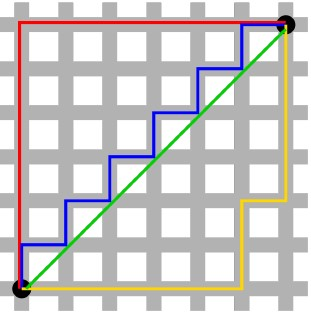
\includegraphics[scale=0.7]{images/manhattan.jpg}
\caption{distance de Manhattan contre distance euclidienne}
\end{figure}

\subsection{Exemple de construction sur un quadrillage}

\begin{minipage}[c]{.6\linewidth}
Toutes les cases du quadrillage sont des sommets et les sommets voisins sont les cases ayant un côté ou un angle commun.\\
Chaque case voisine par le côté est à une distance $10$ soit $1 \times 10$ et les cases en diagonale à une distance $14$ soit $\sqrt{2} \times 10$ arrondi à la valeur entière.\\
\end{minipage}
\hfill %
\begin{minipage}[c]{.35\linewidth}
\begin{center}
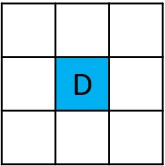
\includegraphics[scale=0.7]{images/quadri1.jpg}
\end{center}
\end{minipage}


On cherche à déterminer le plus court chemin entre D et A.
\begin{center}
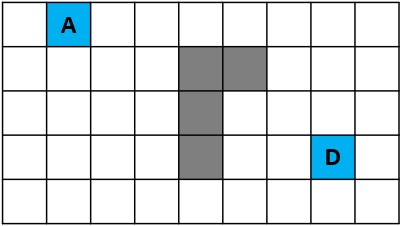
\includegraphics[scale=0.6]{images/quadri2.jpg}
\end{center}

\'Etape 1 : On évalue la distance à l'origine, la distance de la fin et le coût global
\begin{center}
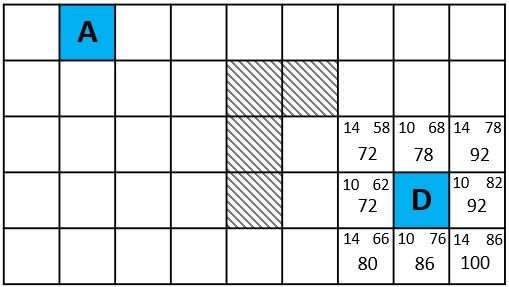
\includegraphics[scale=0.8]{images/quadri3.jpg}
\end{center}

\'Etape 2 : On choisit le sommet dont le coût global est le plus faible. En cas d'égalité, on choisit le sommet le plus proche de l'arrivée.
\begin{center}
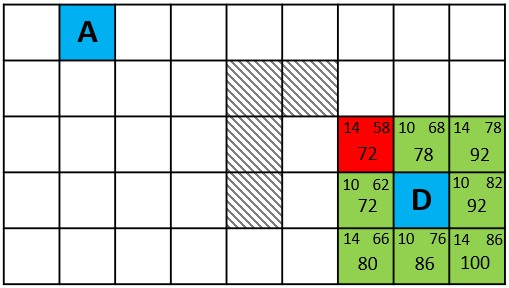
\includegraphics[scale=0.8]{images/quadri4.jpg}
\end{center}

\newpage
\'Etapes 3, 4, 5 et 6:
\begin{center}
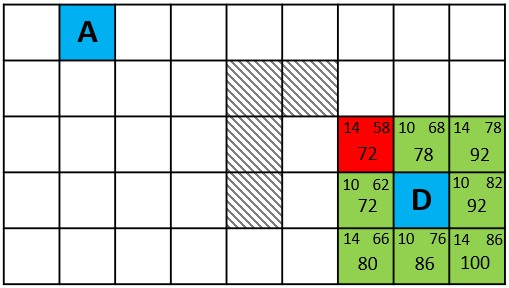
\includegraphics[scale=0.8]{images/quadri4.jpg}
\end{center}

\'Etape 7 :
\begin{center}
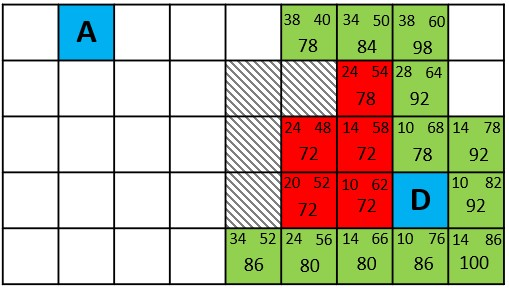
\includegraphics[scale=0.8]{images/quadri9.jpg}
\end{center}


\'Etape 8 :
\begin{center}
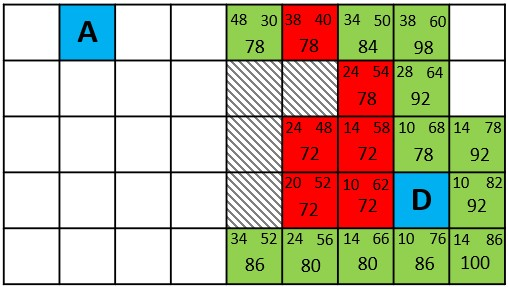
\includegraphics[scale=0.8]{images/quadri10.jpg}
\end{center}

\newpage
\'Etape 9 :
\begin{center}
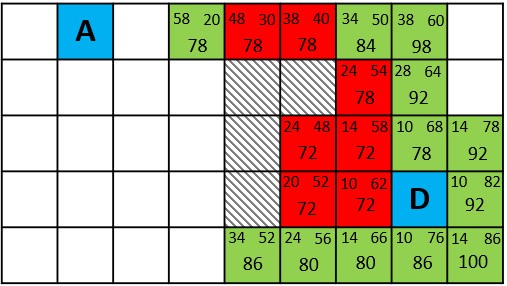
\includegraphics[scale=0.8]{images/quadri11.jpg}
\end{center}

Finalement le chemin le plus court :
\begin{center}
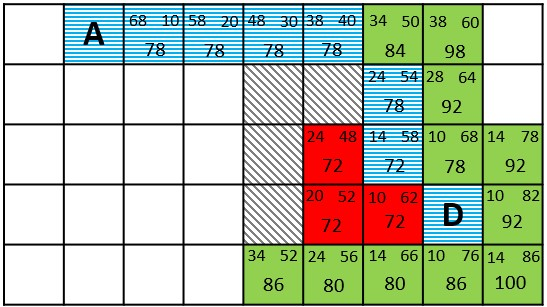
\includegraphics[scale=0.8]{images/quadrifinal.jpg}
\end{center}

\section{Implémentation en python}

\subsection{Structure de données}

Un sommet du graphe peut être représenté sous forme d'une liste dans un dictionnaire avec :
\begin{itemize}
\item la valeur de \texttt{G} (de type \texttt{int}), c'est la distance pour aller du point de départ au sommet considéré ;
\item la valeur de \texttt{H} (de type \texttt{int}), c'est la distance pour aller du sommet considéré au point d'arrivée ;
\item la valeur de \texttt{F} (de type \texttt{int}), c'est la somme des deux précédents mémorisée pour ne pas la recalculer ;
\item le parent, représenté par ses coordonnées.
\end{itemize}

Initialement, un sommet non visité prend comme valeurs :
\{(l,c):\verb![!inf, None, inf, None\verb!]!\}\\
Si le point O(0,0) est le point de départ et A(5,9) est le point d'arrivée, alors le sommet B(0,1) voisin de O prend comme valeurs :\\
\{(0,1):\verb![!10, 106, 116, (0,0)\verb!]!\}\\
On peut aussi choisir l'écriture suivante,\\
\{(0,1):\{'G':10,'H':106,'F':116,'pred' :(0,0)\}\}


\newpage
\subsection{Fonctions à définir}
\subsubsection{L'heuristique}

\begin{python}
\Cache{
def heuristique(pt1:tuple,A:tuple)->int:\\
'''Calcul de la valeur de l'heuristique avec la méthode du cours,
    14 pour un déplacement diagonal et 10 pour un déplacement sur le côté\\
    entrées : pt1, tuple ou list des coordonnées et A, tuple ou list des coordonnées\\
    sortie : H : integer, valeur de l'heuristique '''\\
\indente    a=abs(pt1[0]-A[0])\\
\indente     b=abs(pt1[1]-A[1])\\
\indente     if a<=b:\\
\indente \indente         return (a*14+(b-a)*10)\\
\indente     else:\\
\indente \indente         return (b*14+(a-b)*10)
}
\end{python}


\subsubsection{Le graphe pondéré}

\begin{python}
\Cache{
G=np.ones((5,9))\\
G[1,4]=-10\\
G[1,5]=-10\\
G[2,4]=-10\\
G[3,4]=-10\\
M=\{\}\\
ligne,colonne=G.shape\\
for i in range(ligne):\\
\indente     for j in range(colonne):\\
\indente \indente         if not G[i,j]==-10.0:\\
\indente \indente \indente             M[i,j]=[np.inf,None,np.inf,None]
}
\end{python}

    

\subsubsection{L'algorithme A*}



%\section{Algorithme de A*}

%\vfill
%\textbf{Références :}\\
%P. BEYNET, \textit{Informatique Commune}, Upsti\\
%UPSTI, \textit{Informatique Commune}



\newpage
\renewcommand{\contentsname}{Plan du cours}
\tableofcontents

%\begin{center}
%Vidéo de comparaison des 4 algorithmes de parcours de graphes
%\end{center}
%\begin{center}
%\includegraphics[scale=0.5]{images/qrcode.png}
%\end{center}
%\begin{center}
%https://www.youtube.com/watch?v=GC-nBgi9r0U
%\end{center}



\vfill
\textbf{Références :}\\
https://khayyam.developpez.com/articles/algo/astar/\\
https://www.youtube.com/watch?v=-L-WgKMFuhE

%UPSTI, \textit{Informatique Commune}


\end{document}
